\documentclass{article}
\usepackage{amsmath,amstext,amssymb}
\usepackage[ttscale=0.7]{libertine}
\usepackage[libertine]{newtxmath}
\usepackage{siunitx}
\usepackage{inconsolata}
\usepackage{wrapfig}

\usepackage{sectsty}
\allsectionsfont{\sffamily}

\usepackage{xcolor}
\usepackage[colorlinks=true,
            linkcolor=blue,
            urlcolor=blue,
            breaklinks,
            pdftex,
            allbordercolors=white]{hyperref}
\usepackage{graphicx}
\usepackage{booktabs}
\usepackage[version=4]{mhchem}
\usepackage{parskip}

\usepackage{listings}

\usepackage{datetime2}
\renewcommand{\DTMdisplaydate}[4]{#1-#2-#3}

\begin{document}

\lstset{language=XML,stringstyle=\ttfamily}

\begin{center}
    \Large{\textbf{\sffamily{Setting Up THAMES v2.5 Input}}}
\end{center}
\begin{center}
    \large{Jeffrey W. Bullard}
\end{center}
\begin{center}
    \large{\DTMnow}
\end{center}

\vspace{0.25truein}
\tableofcontents

\vspace{0.25truein}
This document provides guidance on how to prepare input files for THAMES v2.5.  Special
attention is given to common pitfalls to avoid and some troubleshooting recommendations
for fixing improper input files.

\section{Software Requirements}
The following software must be installed and running properly on your computer:
\begin{itemize}
    \item GEM-Selektor 3.6.0 or 3.7.0: \href{http://gems.web.psi.ch/GEMS3/downloads/index.html}{http://gems.web.psi.ch/GEMS3/downloads/index.html}
    \item GEMS3K standalone library 3.4.1: \href{http://gems.web.psi.ch/GEMS3K/downloads/index.html}{http://gems.web.psi.ch/GEMS3K/downloads/index.html}
    \item THAMES v2.5: \href{https://github.tamu.edu/jwbullard/THAMES.git}{https://github.tamu.edu/jwbullard/THAMES.git}
\end{itemize}

\section{Categories of THAMES Input}
Throughout this document, it will be assumed that your THAMES simulation will happen
in a working directory called \verb!$WORKDIR!.

THAMES requires three categories of input files:
\begin{enumerate}
    \item Thermodynamic data input files produced by GEM-Selektor
    \item Microstructure input file and file linking microstructure phases to GEM phases
    \item File to specify calculation times and microstructure output times
    \item (Optional) File containing standard input to redirect to the program
\end{enumerate}
Each of these will be detailed in the following sections.

\subsection{Thermodynamic data input}
This step requires knowledge of how to set up and run a thermodynamic calculation using
GEM-Selektor.

\subsubsection{Data for system}
\begin{wrapfigure}{R}{0.5\textwidth}
    \centering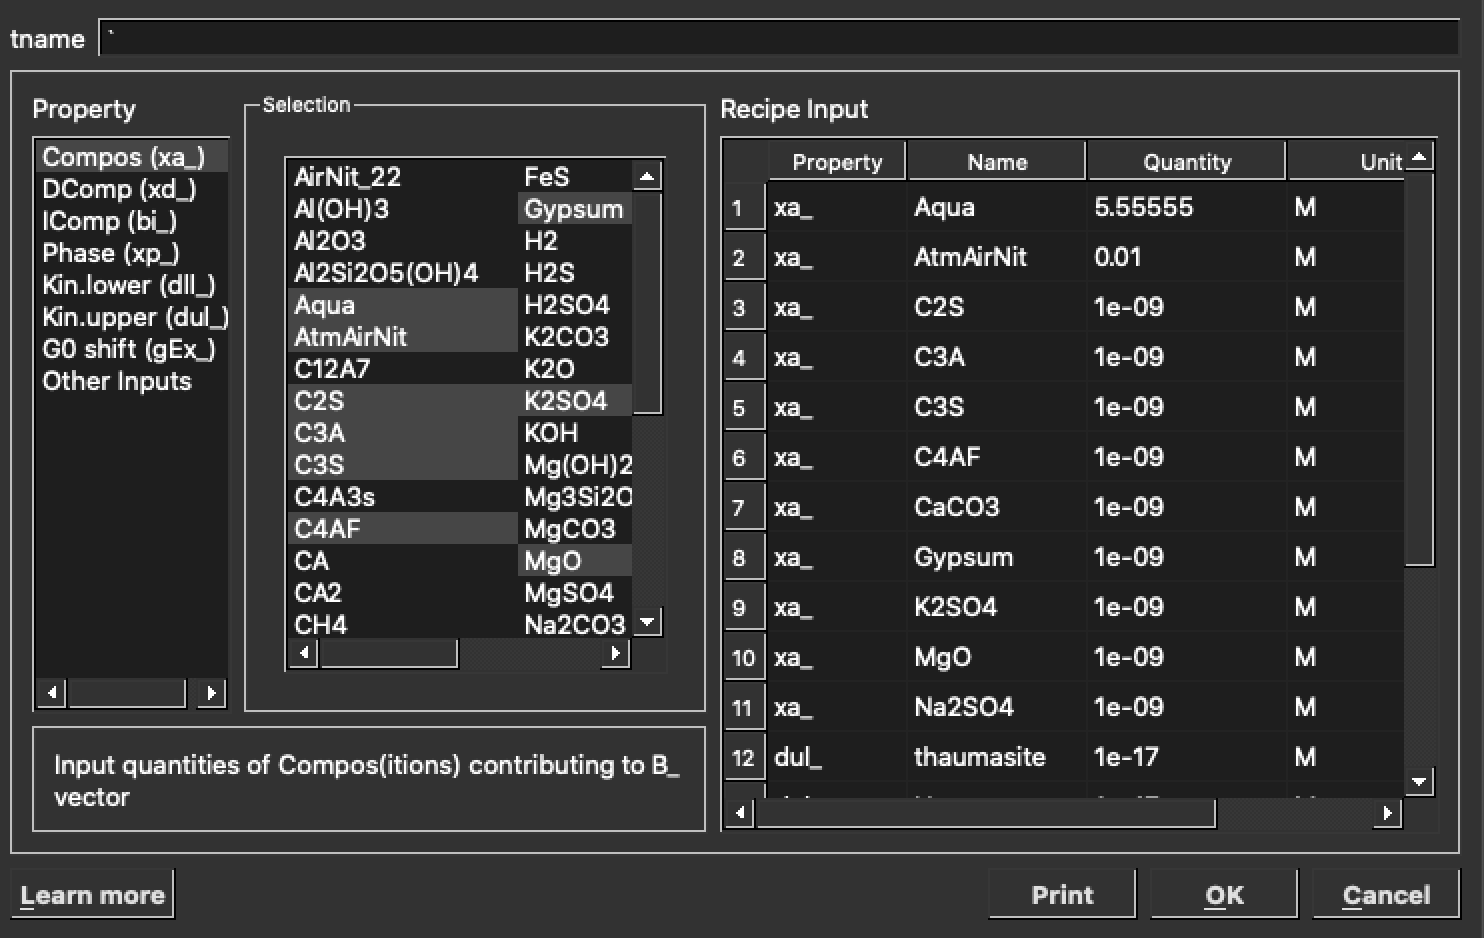
\includegraphics[width=0.45\textwidth]{Figures/GEMrecipe01.png}
    \caption{GEM input recipe for portland cement.}
\end{wrapfigure}

Use GEM-Selektor to construct a recipe for the system of interest, whether it be a portland
cement or other geochemical system.  The actual amounts of each phase or dependent component
do not really matter as long as they are non-zero.  A typical example for portland cement
would be to choose
\SI{5.56}{\mole} of water (\verb!Aqua!) and \SI{0.01}{\mole} of dry normative
air (\verb!AtmAirNit!), and perhaps \SI{1}{\gram} of each of the solid cement
components.  Be sure to place any kinetic upper constraints on phases that are known not to
form in the system.

Run the recipe and accept the result in the dialog window.  Confirm
that the calculation has run without error and produced sensible output.  When you are
confident that the calculation ran smoothly, export the GEMS3K files to \verb!$WORKDIR!:
\begin{verbatim}
Data -> Export GEMS3K files ...
\end{verbatim}
You will need to select a root string for the output files; let us assume that the chosen
root string is \verb!portcem!.  After saving, your \verb!$WORKDIR! will now contain the
following five new files:
\begin{itemize}
    \item \verb!portcem-dat.lst!
    \item \verb!portcem-dbr-0-0000.dat!
    \item \verb!portcem-dbr.lst!
    \item \verb!portcem-dch.dat!
    \item \verb!portcem-ipm.dat!
\end{itemize}

\subsubsection{Data for aqueous solution only}
Next, use GEM-Selektor to clone the system you just made in the previous step, and then
edit its recipe to place an upper kinetic limit of \SI{1e-16}{\mole} on \textsc{every
solid dependent component} (DC) \textit{except} for those  you already have stated in your
recipe.
The purpose of this system is to enable the calculation
of saturation indices of the aqueous solution with respect to the solid dependent components.
The saturation indices play a central role in determining the driving force for dissolution
and precipitation kinetics.

Run this cloned recipe and accept the result in the dialog window.  Confirm
that the calculation has run without error and produced sensible output.  When you are
confident that the calculation ran smoothly, export the GEMS3K files to \verb!$WORKDIR!:
\begin{verbatim}
Data -> Export GEMS3K files ...
\end{verbatim}
As before, you will need to select a root string for the output files; make this be the
same as your previous root string and then add \verb!-sol! to it.  So in this case,
root string is \verb!portcem-sol!.  After saving, your \verb!$WORKDIR! will now contain another
set of five new files:
\begin{itemize}
    \item \verb!portcem-sol-dat.lst!
    \item \verb!portcem-sol-dbr-0-0000.dat!
    \item \verb!portcem-sol-dbr.lst!
    \item \verb!portcem-sol-dch.dat!
    \item \verb!portcem-sol-ipm.dat!
\end{itemize}

Finally, open the file \verb!portcem-sol-dat.lst! with a text editor. It should consist
of one line as follows:
\small{
\begin{verbatim*}
-t "portcem-sol-dch.dat" "portcem-sol-ipm.dat" "portcem-sol-dbr-0-0000.dat"
\end{verbatim*}
}

\normalsize{ }
You must change this to make the first \textit{two} file names be the corresponding file names
of your earlier system; if you followed the instructions so far, you should just remove
the \verb!-sol! string from each of the first two files only:
\small{
\begin{verbatim*}
-t "portcem-dch.dat" "portcem-ipm.dat" "portcem-sol-dbr-0-0000.dat"
\end{verbatim*}
}

\normalsize{ }
\subsubsection{Meaning of GEMS3K the File Contents}
For normal usage of THAMES, one does not need to be concerned with most of the contents of
the GEMS3K files.  However, a few noteworthy items are as follows:
\begin{itemize}
    \item The \verb!-dat.lst! file contains that string that the GEMS3K library reads when
        performing a calculation so that it knows which other files contain the thermodynamic
        data it needs to run.
    \item The \verb!-dch.dat! file contains the names of the independent components
        in the \verb!<ICNL>! field, the names of the dependent components in the
        \verb!<DCNL>! field, and the names of the phases in the \verb!<PHNL>! field.
        You will need these names when correlating microstructure phases with GEM phases.
        This file also contains the parameters needed to calculate the molar volumes
        and densities of the dependent components as a function of temperature and pressure.
    \item The \verb!-dbr.dat! file contains information about the calculated state of
        the system you calculated using GEM Selektor, such as the activity coefficients,
        and phase abundances.  But these will change with subsequent calculations in
        THAMES and so they are not of immediate concern.
    \item The \verb!-ipm.dat! file contains information about the numerical parameters
        used in the calculations, and are not of immediate concern for using THAMES.
\end{itemize}

\fbox{
\begin{minipage}{0.9\textwidth}
    \textbf{WARNING}:  With the sole exception of the modification to the
    \texttt{-sol-dat.lst} file already described, you must \textsc{not} modify
    any of the other GEMS3K input files.  Doing so will likely cause the simulation
    to crash with a GEM error.
\end{minipage}
}

\subsection{Microstructure Files}
\subsubsection{Microstructure phase definitions}
The primary file for specifying microstructure phases and characteristics is given
in an XML file, the schema of which is given in the \verb!chemistry.xsd! file.
We will examine the typical contents of this file for an alite cement paste.

The first several lines prescribe overall characteristics, such as the
temperature, moisture conditions, and water-solids ratio.

\scriptsize{
\begin{lstlisting}
  <numentries>5</numentries>              <!--The number of possible phases-->
  <blaine>403.2</blaine>                  <!--The Blaine fineness in cm2/kg-->
  <refblaine>385.0</refblaine>            <!--Do not change this-->
  <wcRatio>0.36883</wcRatio>              <!--water-solids mass ratio-->
  <temperature>298.15</temperature>       <!--temperature in K-->
  <reftemperature>296.15</reftemperature> <!--Do not change this-->
  <saturated>0</saturated>                <!--1 if saturated, 0 if sealed-->
\end{lstlisting}
}

\normalsize{ }
\fbox{
\begin{minipage}{0.9\textwidth}
    \textbf{WARNING}:  In the current version, the temperature should be the same
    as that contained in the \texttt{-dbr.dat} files.  Changing the temperature will
    not crash the simulation but it will cause the kinetic calculations to be
    inconsistent with the thermodynamic calculations.
\end{minipage}
}

After these initial entries, one can insert an \textbf{optional} section to
specify the initial concentration of solute components, which can be handy for
simulating additives or adjustments to the pH.  The following code shows how
to specify an initial solution with a \ce{H2SO4} concentration of \SI{1.0}{\mol\per\kilogram}.

\scriptsize{
\begin{lstlisting}
  <solution>
    <ICcomp>
    <name>H</name>      <!-- Must be an IC already defined in GEM CSD -->
    <conc>2.0</conc>    <!-- Must be given in molal units, mol/kgw -->
    </ICcomp>
    <ICcomp>
      <name>S</name>
      <conc>1.0</conc>
    </ICcomp>
    <ICcomp>
      <name>O</name>
      <conc>4.0</conc>
    </ICcomp>
  </solution>
\end{lstlisting}
}

\normalsize{ }
\fbox{
\begin{minipage}{0.9\textwidth}
    \textbf{WARNING}:  Composition can be specified using \textbf{only} independent
    components (ICs) that are already defined in your GEM input files described earlier.
    One cannot specify dependent components in the current version, and the concentration
    units must be molal units.
\end{minipage}
}

The remainder of this XML file describes the various
microstructure phases.  The first two phases should always be \verb!Void! and
\verb!H2O!, as shown below:

\scriptsize{
    \begin{lstlisting}
  <!-- Do not change the first two phases here -->
  <phase>
    <thamesname>Void</thamesname>
    <id>0</id>                               <!--ID used in microstructure file-->
    <interface_data>                         <!--Not used for Void phase-->
      <randomgrowth>0.0</randomgrowth>       
    </interface_data>
    <porosity>0.0</porosity>                 <!--Internal fraction of sat pore space-->
    <display_data>                           <!--Display rgb colors, 0 to 255-->
        <red>0.0</red>
        <green>0.0</green>
        <blue>0.0</blue>
        <gray>0.0</gray>
    </display_data>
  </phase>
  <phase>
    <thamesname>H2O</thamesname>             
    <gemphase_data>                          <!--What GEM phase(s) is this?-->
    <gemphasename>aq_gen</gemphasename>      <!--What GEM DCs belongs to this?-->
    <gemdcname>H2O@</gemdcname>
    </gemphase_data>
    <id>1</id>                               <!--ID used in microstructure file-->
    <interface_data>                         <!--Not used for H2O phase-->
      <randomgrowth>0.0</randomgrowth>
    </interface_data>
    <porosity>1.0</porosity>                 <!--Internal fraction of non-solid-->
    <display_data>                           <!--Display rgb colors, 0 to 255-->
      <red>20.0</red>
      <green>20.0</green>
      <blue>25.0</blue>
      <gray>25.0</gray>
    </display_data>
  </phase>
    \end{lstlisting}
}

\normalsize{ }
Following those two microstructure phases, the other phases may have other data fields
such as parameters for kinetic modeling, their relative abundance, and perhaps
multiple GEM phases.  An example for a dissolving portland cement component is
given below:

\scriptsize{
    \begin{lstlisting}
  <phase>
    <thamesname>C3S</thamesname>
    <gemphase_data>
    <gemphasename>Alite</gemphasename>
    <gemdcname>C3S</gemdcname>
    </gemphase_data>
    <id>2</id>                               <!--ID used in microstructure file-->
    <interface_data>
      <randomgrowth>0.0</randomgrowth>       <!--Zero means no randomness-->
      <affinity>
        <affinityphaseid>2</affinityphaseid> <!--Phase interaction with this phase-->
        <affinityvalue>1</affinityvalue>     <!--More positive means more attraction,
                                                  can be negative for repulsion-->
      </affinity>
    </interface_data>
    <porosity>0.0</porosity>                 <!--Internal fraction of non-solid-->
    <impurity_data>                          <!--Impurity data in mol frac-->
      <k2ocoeff>0.00087</k2ocoeff>                 <!--K2O-->
      <na2ocoeff>0.0</na2ocoeff>                   <!--Na2O-->
      <mgocoeff>0.00861</mgocoeff>                 <!--MgO-->
      <so3coeff>0.007942</so3coeff>                <!--SO3-->
    </impurity_data>
    <kinetic_data>
      <type>kinetic</type>                   <!--This phase obeys kinetic model-->
      <scaledmass>100.0</scaledmass>         <!--Mass percentage on total solids basis-->
      <k1>1.5</k1>                           <!--Kinetic model parameters-->
      <k2>0.05</k2>
      <k3>1.1</k3>
      <n1>0.7</n1>
      <n3>3.3</n3>
      <Ea>41570.0</Ea>                       <!--Apparent activation energy-->
      <critdoh>2.0</critdoh>                 <!--Another kinetic model parameter-->
    </kinetic_data>
    <display_data>
      <red>162.0</red>                       <!--Display rgb values, 0 to 255-->
      <green>117.0</green>
      <blue>95.0</blue>
      <gray>220.0</gray>
    </display_data>
  </phase>
    \end{lstlisting}
}

\normalsize{ }
\fbox{
\begin{minipage}{0.9\textwidth}
    \textbf{NOTE}: The \texttt{<id>}values \textsc{must} be in order, starting
    with zero for void and one for water, and then proceeding without
    skipping any numbers.
\end{minipage}
}

An example of a phase that is controlled by thermodynamics rather than
kinetics is \ce{C-S-H}:

\scriptsize{
    \begin{lstlisting}
  <phase>
    <thamesname>CSH</thamesname>
    <gemphase_data>
    <gemphasename>CSHQ</gemphasename>        <!--GEM phase(s) linked to this-->
    <gemdcname>CSHQ-JenD</gemdcname>         <!--GEM DC(s) linked to gemphasename-->
    <gemdcname>CSHQ-JenH</gemdcname>
    <gemdcname>CSHQ-TobD</gemdcname>
    <gemdcname>CSHQ-TobH</gemdcname>
    <gemdcname>KSiOH</gemdcname>
    <gemdcname>NaSiOH</gemdcname>
    </gemphase_data>
    <id>4</id>                               <!--ID used in microstructure file-->
    <interface_data>
      <randomgrowth>0.6</randomgrowth>       <!--Grows in a fairly random manner-->
      <affinity>
        <affinityphaseid>2</affinityphaseid> <!--Same as one of the templates above-->
        <affinityvalue>4</affinityvalue>     <!--More positive means more attraction,
                                                  can be negative for repulsion-->
      </affinity>
      <affinity>
        <affinityphaseid>3</affinityphaseid>
        <affinityvalue>1</affinityvalue> 
      </affinity>
      <affinity>
        <affinityphaseid>4</affinityphaseid>
        <affinityvalue>1</affinityvalue>
      </affinity>
    </interface_data>
    <porosity>0.27</porosity>
    <kinetic_data>
      <type>thermo</type>                    <!--This phase is governed by thermo-->
      <scaledmass>0.0</scaledmass>           <!--No kinetic data needed for thermo phase-->
    </kinetic_data>
    <display_data>                           <!--Display rgb values, 0 to 255-->
      <red>245.0</red>
      <green>222.0</green>
      <blue>179.0</blue>
      <gray>159.0</gray>
    </display_data>
  </phase>

    \end{lstlisting}
}

\normalsize{ }
\fbox{
\begin{minipage}{0.9\textwidth}
    \textbf{NOTE}: Every solid phase \textsc{must} have an \texttt{<affinity>} for
itself, with an \texttt{<affinityvalue>} greater than zero.
\end{minipage}
}

Finally, a phase called \verb!DAMAGE! must \textsc{always} be present, and
should be the final phase in the list.

\scriptsize{
    \begin{lstlisting}
  <phase>
    <thamesname>DAMAGE</thamesname>
    <id>5</id>
    <interface_data>
      <randomgrowth>0.0</randomgrowth>
    </interface_data>
    <porosity>1.0</porosity>
    <display_data>
      <red>255.0</red>
      <green>0.0</green>
      <blue>255.0</blue>
      <gray>255.0</gray>
    </display_data>
  </phase>
    \end{lstlisting}
}

\normalsize{ }
\subsubsection{Rules for linking GEM phases with microstructure phases}
A microstructure phase can be associated with zero, one, or multiple GEM phases;
the user must decide which GEM phase or phases
should be associated with a given microstructure phase.  In some cases the choice
will be obvious, such as identifying \verb!aq_gen! as the saturated pore
liquid in the microstructure.  But in other cases it may be useful or efficient to
group two or more GEM phases into a single microstructure phase.  One example
might be to collect all of the GEM phases associated with carboaluminates, of which
there are many, into a single microstructure phase called \verb!AFm_c! or something
like that, as shown in this example:

\scriptsize{
    \begin{lstlisting}
  <phase>
    <thamesname>MONOSULPH</thamesname>
    <gemphase_data>
        <gemphasename>C4AsH105</gemphasename>
        <gemdcname>monosulphate10.5</gemdcname>
    </gemphase_data>
    <gemphase_data>
        <gemphasename>C4AsH12</gemphasename>
        <gemdcname>monosulphate12</gemdcname>
    </gemphase_data>
    <gemphase_data>
        <gemphasename>C4AsH14</gemphasename>
        <gemdcname>monosulphate14</gemdcname>
    </gemphase_data>
    <gemphase_data>
        <gemphasename>C4AsH9</gemphasename>
        <gemdcname>monosulphate9</gemdcname>
    </gemphase_data>
    <gemphase_data>
        <gemphasename>monosulph-AlFe</gemphasename>
        <gemdcname>monosulphate1205</gemdcname>
        <gemdcname>Fe-monosulph05</gemdcname>
    </gemphase_data>
    <id>13</id>
    <interface_data>
      <randomgrowth>0.6</randomgrowth>
    \end{lstlisting}

    \textit{etc.}

    \begin{lstlisting}
    </phase>
    \end{lstlisting}
}

\normalsize{ }
Whatever choices are made, both the GEM phase name and the names of all
the DC components for that phase must be placed within \verb!<gemphase_data>! field,
and there must be one of these fields for each GEM phase that you wish to link
to the microstructure phase.  In addition, the \verb!gemphasename! must exactly match
one of the \verb!<PHNL>! entries in the \verb!-dch.dat! file, and
\textit{all} of the DCs associated with that phase must immediately follow that
phase as shown in this example.  Determine which GEM DCs are associated
with a given phase by consulting the \verb!<nDCinPH>! field of the \verb!-dch.dat! file.

To illustrate, Figure~\ref{fig:dchfile} shows a portion of a real \verb!-dch.dat! file.
In the figure, there are \textit{nine} phases listed in the \verb!<PHNL>! field and
26 DCs listed in the \verb!<DCNL>! field.  The numbers in the \verb!<nDCinPH>! field
relate the two.  Notice that there are \textit{nine} numbers in \verb!<nDCinPH>!, one
for each phase. The ordering of the numbers is the same as the ordering of phase
names in the \verb!<PHNL>! field.  So there are 13 DCs in the first phase, which
is \verb!<aq_gen>!.  In addition, those 13 DCs are the \textit{first} 13 DCs in the
\verb!<DCNL>! list.  Moving on, we see that there are three DCs in the next phase, which
is \verb!gas_gen!, and those three DCs are the next three after the first 13 in the
\verb!<DCNL>! list, namely \verb!'H2'!, \verb!'O2'!, and \verb!'H2O'! (the last being
the water vapor molecule, not liquid water which is \verb!H2O@!\footnote{In GEMS, the
\makeatletter\texttt{`@'}\makeatother\ symbol is reserved to designate
a zero-charge liquid solvent or
a zero-charge dissolved component.  Gas molecules do not have this symbol even though
they also have zero charge.}

\begin{figure}
    \centering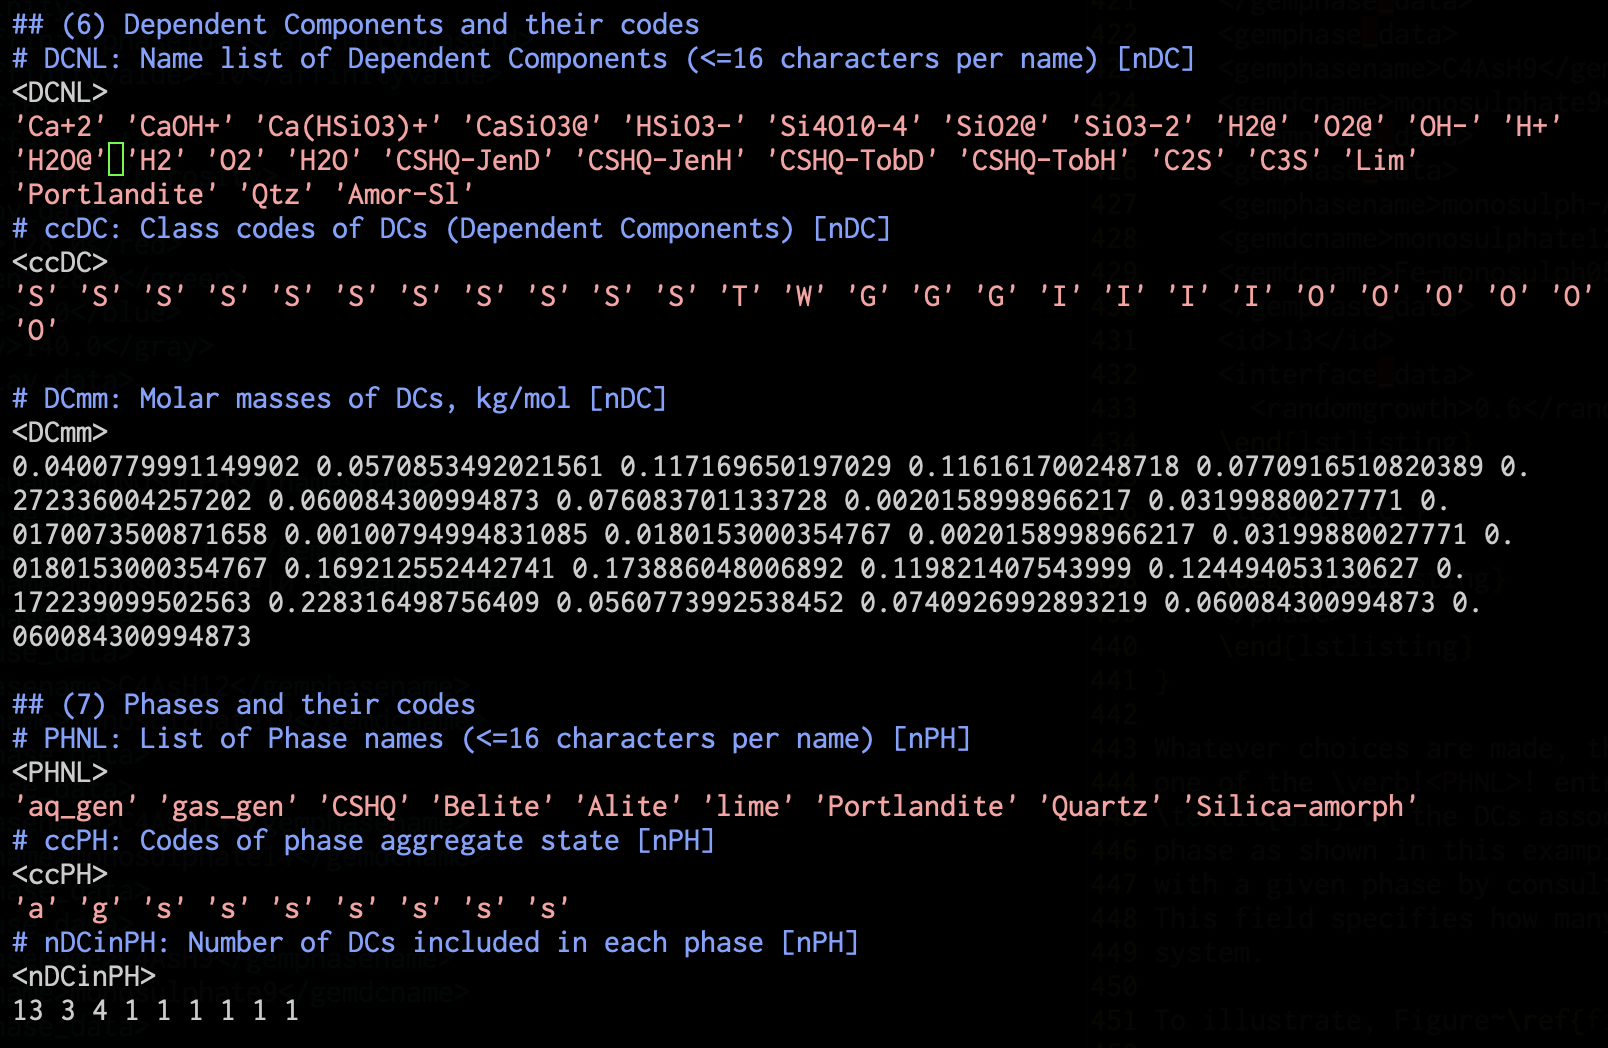
\includegraphics[width=0.7\textwidth]{Figures/dchfile.png}
    \caption{\label{fig:dchfile} Portion of a DCH input file showing the definitions
    of GEM phases and DCs.}
\end{figure}

\subsubsection{Microstructure initial 3D arrangement}
The microstructure representation is a digitized 3D image with \verb!X_Size! voxels
in the $x$ direction, \verb!Y_Size! in the $y$ direction, and \verb!Z_Size!
in the $z$ direction.  Each voxel is a physical dimension of
\verb!Image_Resolution! in micrometer units.
This is a normal ASCII text file.  The first few lines of an example microstructure
are given below.

\small{
\begin{verbatim*}
Version: 5.0
X_Size: 100
Y_Size: 100
Z_Size: 100
Image_Resolution: 1.0
1
1
1
2
1
2
1
\end{verbatim*}
}

\normalsize{ }
Note that the \verb!Version! descriptor is not currently used.  After the five-line
header to this file, each line contains a single integer corresponding to the ID of
one of the microstructure phases (not the GEM phases).  The rows have a
\verb!z-y-x! nesting convention, by the first voxel is $(0,0,0)$, the $x$ coordinates
vary most quickly and the $z$ coordinates vary most slowly.

One way to generate such a file is to create a virtual 3D microstructure using VCCTL,
which produces a \verb!.img! file in much the same format as just shown.  However,
the VCCTL phase ID numbers (Table~\ref{tab:vcctlphases}) are different than the
ones required by THAMES.  Therefore, one must replace
the VCCTL ID numbers with the corresponding THAMES microstructure id numbers.
A C program called \verb!vcctl2thames! has been provided to assist with this, but the
program may need to be edited as needed to be consistent with the THAMES microstructure
definition file (\verb!chemistry.xml!).

\small{
\begin{table}
    \caption{\label{tab:vcctlphases} VCCTL 9.5 phase identification numbers}
\begin{tabular}{lSlSls} \toprule
    Phase & \multicolumn{1}{c}{ID} &
    Phase & \multicolumn{1}{c}{ID} &
    Phase & \multicolumn{1}{c}{ID} \\ \midrule
    Water & 0 & Gypsum & 7 & \ce{Ca(OH)2} & 19 \\
    Void & 55 & Bassanite (Hemihydrate) & 8 & \ce{C-S-H} & 20 \\
    Alite & 1 & Anhydrite (\ce{CaSO4}) & 9 & \ce{C3AH6} & 21 \\
    Belite & 2 & Silica Fume & 10 & Ettringite & 22 \\
    \ce{C3A} & 3 & Inert & 11 & \ce{Fe(OH)3} & 25 \\
    \ce{C4AF} & 4 & Silica glass & 16 & Pozzolanic \ce{C-S-H} & 26 \\
    \ce{K2SO4} & 5 & Monosulfate & 24 & Friedel salt & 29 \\
    \ce{Na2SO4} & 6 & Monocarboaluminate & 34 & \ce{CaCl2} & 28 \\
    \ce{CaCO3} & 33 & Str{\"{a}}tlingite & 30 & Brucite & 35 \\ \bottomrule
\end{tabular}
\end{table}
}

\normalsize{}
\subsection{Calculation and Output Times}
The file for specifying calculation times and output times
is an XML file, the schema of which is given in the \verb!parameters.xsd! file.
Each calculation time is specified (in days) with a line like this:

\small{
\begin{lstlisting}
<calctime>0.001331</calctime>
\end{lstlisting}
}

\normalsize{ }
Generally, it is a good idea to have a lot of calculation times using closely
spaced time intervals, especially at early times.  This is needed to prevent the
kinetic changes during any time interval from being so large that the thermodynamic
equilibrium calculations cannot converge.

After all the calculation times have been specified, the user can specify any
number of simulation times (in days) at which to output a 3D microstructure image.
The syntax for this is

\small{
\begin{lstlisting}
<outtime>28.0</outtime>
\end{lstlisting}
}

\end{document}
